% generated by src/r2/paper_assets (make_paper_assets.py figures); do not edit by hand
% provenance: fig7_hubs generated by src/r2/paper_assets on 2026-10-15 04:07 from data/r2/tables/
%   heldout_degree_calibration.csv (modified 2026-10-14 20:08): reference in {encode, enets2, pert_pooled}; (score, set) in (family_hb, strong_bfdr05), (em, top500), (fisher, top500), (dorothea_level_heldin, top500), (random, top500)
%   sim_hub_summary.csv (modified 2026-10-14 20:37): set_rule = size_matched, metric in {over_promotion_lit_q5, over_promotion_top_decile}; methods oracle, family_hb, em, dependence, fisher, stouffer, majority, union, vote_fraction; set_rule = size_matched, metric = set_size, method = family_hb
%   (constants): FEW_TFS from r2.heldout_eval
\begin{figure}[tbp]
  \centering
  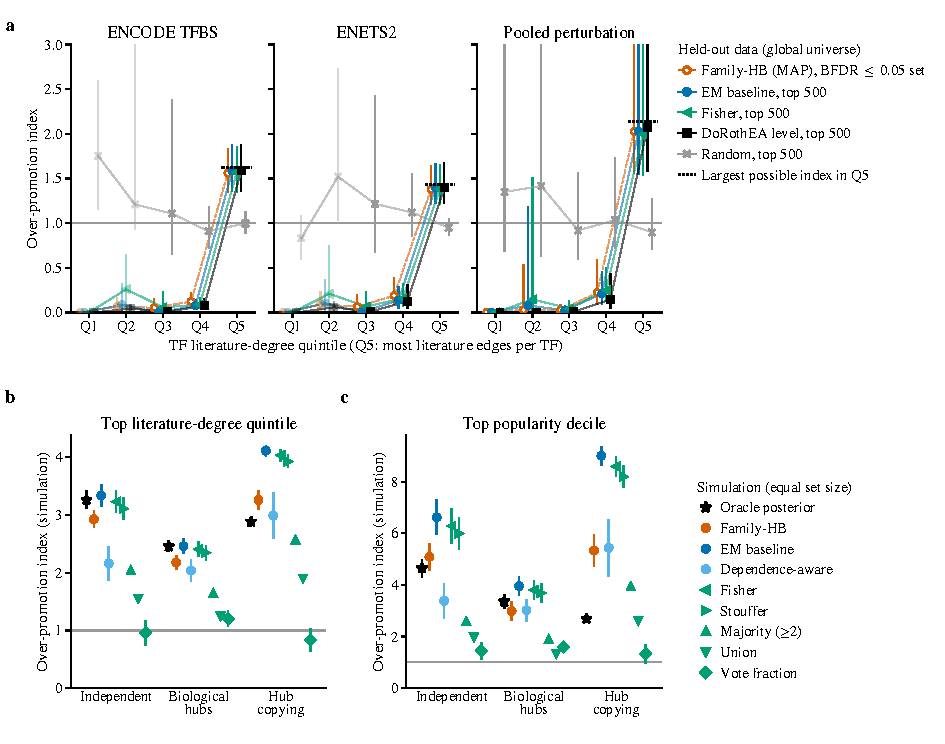
\includegraphics[width=\textwidth]{fig7_hubs.pdf}
  \caption{\textbf{Over-promotion of well-studied TFs.} The over-promotion index of a selected set for a group of TFs is the share of the set in the group divided by the share of positives (a) or of true edges (b, c) in the group (1: proportional to the positives; in (b, c) the oracle posterior shows the level the evidence supports). (a) Held-out data, global universe: index by quintile of TF literature degree for the Family-HB (MAP) BFDR $\leq 0.05$ set and for the top 500 edges of selected scores, with 95\% TF-bootstrap intervals holding the set fixed (faded (post hoc): fewer than 5 evaluable TFs in the quintile). Literature edges per TF in quintiles Q1--Q5: 1--2, 3--6, 7--17, 18--54, 55--1{,}444. The top quintile holds 96\% of the Family-HB set but 62\% of ENCODE positives; index of the Family-HB set in the top quintile: ENCODE 1.56 [1.34, 1.84], ENETS2 1.38 [1.20, 1.65], pooled perturbation 2.03 [1.55, 3.11]; random top 500 on ENCODE: 1.00 [0.88, 1.13]. In the top quintile the index cannot exceed 1/(share of positives) (dotted; ENCODE TFBS 1.62; ENETS2 1.43; Pooled perturbation 2.14), so every informative score is near this ceiling and panel (a) does not separate estimators; the sets also differ in size. (b, c) Simulation with known truth (20 replicates per scenario; mean with 95\% interval over replicates): index of sets of the size of the Family-HB BFDR $\leq 0.05$ set at TFs in the top literature-degree quintile (b) and in the top popularity decile (c), relative to the true edges. Under hub-concentrated copying (b): oracle posterior 2.89 [2.80, 2.97], Family-HB 3.26 [3.10, 3.42], EM 4.11 [4.02, 4.20], Fisher 4.03 [3.93, 4.14]. Family-regularized coincides with EM to two decimals and is not shown. All simulation rows are post hoc.}
  \label{fig:hubs}
\end{figure}
